\documentclass[10pt, twoside, twocolumn]{book}
\usepackage[utf8]{inputenc}

\usepackage[left=1cm, right=1cm, top=1cm, bottom=1cm, portrait, a4paper]{geometry}
\setlength{\columnsep}{1cm}

\usepackage[parfill]{parskip}    % Activate to begin paragraphs with an empty line rather than an indent

\usepackage{graphicx}
\usepackage{amssymb}
\usepackage{epstopdf}

\usepackage{framed}

\usepackage{fancyhdr}
\pagestyle{fancy}
\fancyhead{} % clear all header fields
%\fancyhead[LO,LE]{\Large \thetitle}
\fancyfoot{} % clear all footer fields
\fancyfoot[RE,RO]{}%{\thepage}
%\fancyfoot[LO,LE]{Reactive Systems Engineering 2013}
\renewcommand{\headrulewidth}{0pt}% 1pt
\renewcommand{\footrulewidth}{0pt}% 1pt

%\newcommand{\tightlist}{}
\providecommand{\tightlist}{%
  \setlength{\itemsep}{0pt}\setlength{\parskip}{0pt}}

\renewcommand{\labelitemi}{--}
\usepackage{enumerate}

%\usepackage[pdftex]{changebar}

\usepackage{amssymb}

\usepackage{url}
%\usepackage[hyphens]{url}
\usepackage[breaklinks]{hyperref}
\urlstyle{same}
\hypersetup{
    colorlinks=true,
    linkcolor=blue,
    filecolor=magenta,      
    urlcolor=cyan,
}


\usepackage{aeguill}

\usepackage{multicol}
\usepackage[usenames]{xcolor}
\definecolor{gray}{rgb}{.3,.3,.3}

\DeclareGraphicsRule{.tif}{png}{.png}{`convert #1 `dirname #1`/`basename #1 .tif`.png}

\usepackage{tabularx}
\usepackage{booktabs}
\usepackage{longtable}
\usepackage{tabulary}
\usepackage[normalem]{ulem}

\usepackage{fvextra}
\DefineShortVerb[commandchars=\\\{\}]{\|}
\DefineVerbatimEnvironment{Highlighting}{Verbatim}{commandchars=\\\{\}}
% Add ',fontsize=\small' for more characters per line
\newenvironment{Shaded}{}{}
\newcommand{\KeywordTok}[1]{\textcolor[rgb]{0.00,0.44,0.13}{\textbf{{#1}}}}
\newcommand{\DataTypeTok}[1]{\textcolor[rgb]{0.56,0.13,0.00}{{#1}}}
\newcommand{\DecValTok}[1]{\textcolor[rgb]{0.25,0.63,0.44}{{#1}}}
\newcommand{\BaseNTok}[1]{\textcolor[rgb]{0.25,0.63,0.44}{{#1}}}
\newcommand{\FloatTok}[1]{\textcolor[rgb]{0.25,0.63,0.44}{{#1}}}
\newcommand{\CharTok}[1]{\textcolor[rgb]{0.25,0.44,0.63}{{#1}}}
\newcommand{\StringTok}[1]{\textcolor[rgb]{0.25,0.44,0.63}{{#1}}}
\newcommand{\CommentTok}[1]{\textcolor[rgb]{0.38,0.63,0.69}{\textit{{#1}}}}
\newcommand{\OtherTok}[1]{\textcolor[rgb]{0.00,0.44,0.13}{{#1}}}
\newcommand{\AlertTok}[1]{\textcolor[rgb]{1.00,0.00,0.00}{\textbf{{#1}}}}
\newcommand{\FunctionTok}[1]{\textcolor[rgb]{0.02,0.16,0.49}{{#1}}}
\newcommand{\RegionMarkerTok}[1]{{#1}}
\newcommand{\ErrorTok}[1]{\textcolor[rgb]{1.00,0.00,0.00}{\textbf{{#1}}}}
\newcommand{\NormalTok}[1]{{#1}}
\newcommand{\BuiltInTok}[1]{{#1}}
\newcommand{\ExtensionTok}[1]{{#1}}
\newcommand{\ImportTok}[1]{{#1}}
\newcommand{\OperatorTok}[1]{{#1}}
\newcommand{\ControlFlowTok}[1]{{#1}}
\newcommand{\SpecialCharTok}[1]{{#1}}
\newcommand{\VariableTok}[1]{{#1}}


%\usepackage{helvet}
%\usepackage{charter}
%\renewcommand{\sfdefault}{phv}

\usepackage[absolute]{textpos}
\setlength{\TPHorizModule}{40mm}
\setlength{\TPVertModule}{10mm}
\textblockorigin{20mm}{20mm} % start everything near the top-left corner


\usepackage{enumitem}

\LetLtxMacro{\OldIncludegraphics}{\includegraphics}
\renewcommand{\includegraphics}[2][]{\OldIncludegraphics[width=\linewidth, #1]{#2}}
\renewcommand{\caption}{}

\usepackage{ifthen}

\newcommand{\nbox}[1]{%
\setlength{\fboxsep}{2pt}
\setlength{\fboxrule}{0.4pt}
\framebox[0.3in][r]{\raisebox{-0.8cm}{\small\textsf{#1}}}}

\newcommand{\teamprefix}[4]{%
% #1 team number
% #2 course
% #3 rat
% #4 date
\vspace*{5cm}%
\begin{center}
\begin{minipage}{0.5\linewidth}
\emph{Keep the scratch card attached to the paper and hand in both of them.}
\end{minipage}
\end{center}
\vspace*{5cm}%
\addthumb{}{#1}{white}{black}
\begin{tabular}{@{}ll}%
\ifthenelse{\not\equal{#2}{}}{Course: & \textbf{#2}\\}{}%
RAT: & \textbf{#3} \\
\ifthenelse{\not\equal{#4}{}}{Date: & \textbf{#4}\\}{}%
Team: & \textbf{#1}\\
\end{tabular}\\%
\rule{\linewidth}{0.4pt}
\vfill
}%

\newcommand{\individualprefix}[7]{%
% #1 name
% #2 name shortcode
% #3 team number
% #4 table (optional)
% #5 course
% #6 rat
% #7 date
\begin{tabular}{@{}ll}
\ifthenelse{\not\equal{#5}{}}{Course: & \textbf{#5}\\}{}%
RAT: & \textbf{#6} \\
\ifthenelse{\not\equal{#7}{}}{Date: & \textbf{#7}\\}{}%
      &   \\
Name: & \textbf{#1} --- \texttt{#2}\\
Team: & \textbf{#3} \\
\ifthenelse{\not\equal{#4}{}}{Table: & \textbf{#4}\\}{}%
\end{tabular}\vspace{1em}

%
\rule{\linewidth}{0.4pt}
\textsf{\textbf{Instructions:}}
\begin{itemize}\setlength\itemsep{-0.5em}
\item Select \textbf{one} answer alternative for each question.
\item Select the answer alternative that matches \textbf{best}.
\item No helping material is allowed.
\item Only write within the answer box.
\end{itemize}
%
\rule{\linewidth}{0.4pt}
\textsf{\textbf{Answers:} (A, B, C, or D)}\\
\begin{tabularx}{\linewidth}{@{}XXXXXXXXXX}
\nbox{1}&\nbox{2}&\nbox{3}&\nbox{4}&\nbox{5}&\nbox{6}&\nbox{7}&\nbox{8}&\nbox{9}&\nbox{10}\\
\end{tabularx}\\

\textsf{\textbf{Checksum:} (Count how many of each letters you have used.)}\\
\begin{tabularx}{\linewidth}{@{}XXXXXXXXXX}
\nbox{A} & \nbox{B} & \nbox{C} & \nbox{D}   & & & & & & \\
\end{tabularx}
\vfill
}%

% pandoc creates figures that float away, so we override and set position to H.
% Overwrite \begin{figure}[htbp] with \begin{figure}[H]
\usepackage{float}
\let\origfigure=\figure
\let\endorigfigure=\endfigure
\renewenvironment{figure}[1][]{%
  \origfigure[H]
}{%
  \endorigfigure
}

\usepackage[sfdefault]{biolinum}

\newcommand{\question}[1]{
\vspace{10pt}
\vfill
\rule{\linewidth}{0.4pt}
\textsf{\textbf{Question #1:}}
}

\usepackage[width=0.8cm]{thumbs}


\makeatletter
\def\PY@reset{\let\PY@it=\relax \let\PY@bf=\relax%
    \let\PY@ul=\relax \let\PY@tc=\relax%
    \let\PY@bc=\relax \let\PY@ff=\relax}
\def\PY@tok#1{\csname PY@tok@#1\endcsname}
\def\PY@toks#1+{\ifx\relax#1\empty\else%
    \PY@tok{#1}\expandafter\PY@toks\fi}
\def\PY@do#1{\PY@bc{\PY@tc{\PY@ul{%
    \PY@it{\PY@bf{\PY@ff{#1}}}}}}}
\def\PY#1#2{\PY@reset\PY@toks#1+\relax+\PY@do{#2}}

\expandafter\def\csname PY@tok@w\endcsname{\def\PY@tc##1{\textcolor[rgb]{0.73,0.73,0.73}{##1}}}
\expandafter\def\csname PY@tok@c\endcsname{\let\PY@it=\textit\def\PY@tc##1{\textcolor[rgb]{0.25,0.50,0.50}{##1}}}
\expandafter\def\csname PY@tok@cp\endcsname{\def\PY@tc##1{\textcolor[rgb]{0.74,0.48,0.00}{##1}}}
\expandafter\def\csname PY@tok@k\endcsname{\let\PY@bf=\textbf\def\PY@tc##1{\textcolor[rgb]{0.00,0.50,0.00}{##1}}}
\expandafter\def\csname PY@tok@kp\endcsname{\def\PY@tc##1{\textcolor[rgb]{0.00,0.50,0.00}{##1}}}
\expandafter\def\csname PY@tok@kt\endcsname{\def\PY@tc##1{\textcolor[rgb]{0.69,0.00,0.25}{##1}}}
\expandafter\def\csname PY@tok@o\endcsname{\def\PY@tc##1{\textcolor[rgb]{0.40,0.40,0.40}{##1}}}
\expandafter\def\csname PY@tok@ow\endcsname{\let\PY@bf=\textbf\def\PY@tc##1{\textcolor[rgb]{0.67,0.13,1.00}{##1}}}
\expandafter\def\csname PY@tok@nb\endcsname{\def\PY@tc##1{\textcolor[rgb]{0.00,0.50,0.00}{##1}}}
\expandafter\def\csname PY@tok@nf\endcsname{\def\PY@tc##1{\textcolor[rgb]{0.00,0.00,1.00}{##1}}}
\expandafter\def\csname PY@tok@nc\endcsname{\let\PY@bf=\textbf\def\PY@tc##1{\textcolor[rgb]{0.00,0.00,1.00}{##1}}}
\expandafter\def\csname PY@tok@nn\endcsname{\let\PY@bf=\textbf\def\PY@tc##1{\textcolor[rgb]{0.00,0.00,1.00}{##1}}}
\expandafter\def\csname PY@tok@ne\endcsname{\let\PY@bf=\textbf\def\PY@tc##1{\textcolor[rgb]{0.82,0.25,0.23}{##1}}}
\expandafter\def\csname PY@tok@nv\endcsname{\def\PY@tc##1{\textcolor[rgb]{0.10,0.09,0.49}{##1}}}
\expandafter\def\csname PY@tok@no\endcsname{\def\PY@tc##1{\textcolor[rgb]{0.53,0.00,0.00}{##1}}}
\expandafter\def\csname PY@tok@nl\endcsname{\def\PY@tc##1{\textcolor[rgb]{0.63,0.63,0.00}{##1}}}
\expandafter\def\csname PY@tok@ni\endcsname{\let\PY@bf=\textbf\def\PY@tc##1{\textcolor[rgb]{0.60,0.60,0.60}{##1}}}
\expandafter\def\csname PY@tok@na\endcsname{\def\PY@tc##1{\textcolor[rgb]{0.49,0.56,0.16}{##1}}}
\expandafter\def\csname PY@tok@nt\endcsname{\let\PY@bf=\textbf\def\PY@tc##1{\textcolor[rgb]{0.00,0.50,0.00}{##1}}}
\expandafter\def\csname PY@tok@nd\endcsname{\def\PY@tc##1{\textcolor[rgb]{0.67,0.13,1.00}{##1}}}
\expandafter\def\csname PY@tok@s\endcsname{\def\PY@tc##1{\textcolor[rgb]{0.73,0.13,0.13}{##1}}}
\expandafter\def\csname PY@tok@sd\endcsname{\let\PY@it=\textit\def\PY@tc##1{\textcolor[rgb]{0.73,0.13,0.13}{##1}}}
\expandafter\def\csname PY@tok@si\endcsname{\let\PY@bf=\textbf\def\PY@tc##1{\textcolor[rgb]{0.73,0.40,0.53}{##1}}}
\expandafter\def\csname PY@tok@se\endcsname{\let\PY@bf=\textbf\def\PY@tc##1{\textcolor[rgb]{0.73,0.40,0.13}{##1}}}
\expandafter\def\csname PY@tok@sr\endcsname{\def\PY@tc##1{\textcolor[rgb]{0.73,0.40,0.53}{##1}}}
\expandafter\def\csname PY@tok@ss\endcsname{\def\PY@tc##1{\textcolor[rgb]{0.10,0.09,0.49}{##1}}}
\expandafter\def\csname PY@tok@sx\endcsname{\def\PY@tc##1{\textcolor[rgb]{0.00,0.50,0.00}{##1}}}
\expandafter\def\csname PY@tok@m\endcsname{\def\PY@tc##1{\textcolor[rgb]{0.40,0.40,0.40}{##1}}}
\expandafter\def\csname PY@tok@gh\endcsname{\let\PY@bf=\textbf\def\PY@tc##1{\textcolor[rgb]{0.00,0.00,0.50}{##1}}}
\expandafter\def\csname PY@tok@gu\endcsname{\let\PY@bf=\textbf\def\PY@tc##1{\textcolor[rgb]{0.50,0.00,0.50}{##1}}}
\expandafter\def\csname PY@tok@gd\endcsname{\def\PY@tc##1{\textcolor[rgb]{0.63,0.00,0.00}{##1}}}
\expandafter\def\csname PY@tok@gi\endcsname{\def\PY@tc##1{\textcolor[rgb]{0.00,0.63,0.00}{##1}}}
\expandafter\def\csname PY@tok@gr\endcsname{\def\PY@tc##1{\textcolor[rgb]{1.00,0.00,0.00}{##1}}}
\expandafter\def\csname PY@tok@ge\endcsname{\let\PY@it=\textit}
\expandafter\def\csname PY@tok@gs\endcsname{\let\PY@bf=\textbf}
\expandafter\def\csname PY@tok@gp\endcsname{\let\PY@bf=\textbf\def\PY@tc##1{\textcolor[rgb]{0.00,0.00,0.50}{##1}}}
\expandafter\def\csname PY@tok@go\endcsname{\def\PY@tc##1{\textcolor[rgb]{0.53,0.53,0.53}{##1}}}
\expandafter\def\csname PY@tok@gt\endcsname{\def\PY@tc##1{\textcolor[rgb]{0.00,0.27,0.87}{##1}}}
\expandafter\def\csname PY@tok@err\endcsname{\def\PY@bc##1{\setlength{\fboxsep}{0pt}\fcolorbox[rgb]{1.00,0.00,0.00}{1,1,1}{\strut ##1}}}
\expandafter\def\csname PY@tok@kc\endcsname{\let\PY@bf=\textbf\def\PY@tc##1{\textcolor[rgb]{0.00,0.50,0.00}{##1}}}
\expandafter\def\csname PY@tok@kd\endcsname{\let\PY@bf=\textbf\def\PY@tc##1{\textcolor[rgb]{0.00,0.50,0.00}{##1}}}
\expandafter\def\csname PY@tok@kn\endcsname{\let\PY@bf=\textbf\def\PY@tc##1{\textcolor[rgb]{0.00,0.50,0.00}{##1}}}
\expandafter\def\csname PY@tok@kr\endcsname{\let\PY@bf=\textbf\def\PY@tc##1{\textcolor[rgb]{0.00,0.50,0.00}{##1}}}
\expandafter\def\csname PY@tok@bp\endcsname{\def\PY@tc##1{\textcolor[rgb]{0.00,0.50,0.00}{##1}}}
\expandafter\def\csname PY@tok@fm\endcsname{\def\PY@tc##1{\textcolor[rgb]{0.00,0.00,1.00}{##1}}}
\expandafter\def\csname PY@tok@vc\endcsname{\def\PY@tc##1{\textcolor[rgb]{0.10,0.09,0.49}{##1}}}
\expandafter\def\csname PY@tok@vg\endcsname{\def\PY@tc##1{\textcolor[rgb]{0.10,0.09,0.49}{##1}}}
\expandafter\def\csname PY@tok@vi\endcsname{\def\PY@tc##1{\textcolor[rgb]{0.10,0.09,0.49}{##1}}}
\expandafter\def\csname PY@tok@vm\endcsname{\def\PY@tc##1{\textcolor[rgb]{0.10,0.09,0.49}{##1}}}
\expandafter\def\csname PY@tok@sa\endcsname{\def\PY@tc##1{\textcolor[rgb]{0.73,0.13,0.13}{##1}}}
\expandafter\def\csname PY@tok@sb\endcsname{\def\PY@tc##1{\textcolor[rgb]{0.73,0.13,0.13}{##1}}}
\expandafter\def\csname PY@tok@sc\endcsname{\def\PY@tc##1{\textcolor[rgb]{0.73,0.13,0.13}{##1}}}
\expandafter\def\csname PY@tok@dl\endcsname{\def\PY@tc##1{\textcolor[rgb]{0.73,0.13,0.13}{##1}}}
\expandafter\def\csname PY@tok@s2\endcsname{\def\PY@tc##1{\textcolor[rgb]{0.73,0.13,0.13}{##1}}}
\expandafter\def\csname PY@tok@sh\endcsname{\def\PY@tc##1{\textcolor[rgb]{0.73,0.13,0.13}{##1}}}
\expandafter\def\csname PY@tok@s1\endcsname{\def\PY@tc##1{\textcolor[rgb]{0.73,0.13,0.13}{##1}}}
\expandafter\def\csname PY@tok@mb\endcsname{\def\PY@tc##1{\textcolor[rgb]{0.40,0.40,0.40}{##1}}}
\expandafter\def\csname PY@tok@mf\endcsname{\def\PY@tc##1{\textcolor[rgb]{0.40,0.40,0.40}{##1}}}
\expandafter\def\csname PY@tok@mh\endcsname{\def\PY@tc##1{\textcolor[rgb]{0.40,0.40,0.40}{##1}}}
\expandafter\def\csname PY@tok@mi\endcsname{\def\PY@tc##1{\textcolor[rgb]{0.40,0.40,0.40}{##1}}}
\expandafter\def\csname PY@tok@il\endcsname{\def\PY@tc##1{\textcolor[rgb]{0.40,0.40,0.40}{##1}}}
\expandafter\def\csname PY@tok@mo\endcsname{\def\PY@tc##1{\textcolor[rgb]{0.40,0.40,0.40}{##1}}}
\expandafter\def\csname PY@tok@ch\endcsname{\let\PY@it=\textit\def\PY@tc##1{\textcolor[rgb]{0.25,0.50,0.50}{##1}}}
\expandafter\def\csname PY@tok@cm\endcsname{\let\PY@it=\textit\def\PY@tc##1{\textcolor[rgb]{0.25,0.50,0.50}{##1}}}
\expandafter\def\csname PY@tok@cpf\endcsname{\let\PY@it=\textit\def\PY@tc##1{\textcolor[rgb]{0.25,0.50,0.50}{##1}}}
\expandafter\def\csname PY@tok@c1\endcsname{\let\PY@it=\textit\def\PY@tc##1{\textcolor[rgb]{0.25,0.50,0.50}{##1}}}
\expandafter\def\csname PY@tok@cs\endcsname{\let\PY@it=\textit\def\PY@tc##1{\textcolor[rgb]{0.25,0.50,0.50}{##1}}}

\def\PYZbs{\char`\\}
\def\PYZus{\char`\_}
\def\PYZob{\char`\{}
\def\PYZcb{\char`\}}
\def\PYZca{\char`\^}
\def\PYZam{\char`\&}
\def\PYZlt{\char`\<}
\def\PYZgt{\char`\>}
\def\PYZsh{\char`\#}
\def\PYZpc{\char`\%}
\def\PYZdl{\char`\$}
\def\PYZhy{\char`\-}
\def\PYZsq{\char`\'}
\def\PYZdq{\char`\"}
\def\PYZti{\char`\~}
% for compatibility with earlier versions
\def\PYZat{@}
\def\PYZlb{[}
\def\PYZrb{]}
\makeatother



\begin{document}
\pagenumbering{arabic}
\chapter{Unit 1 — State Machines}
\hypertarget{state-machines}{%
\section{State Machines}\label{state-machines}}

In the previous units, we learned how to capture and understand our
user's requirements for a system, and structure the functionality that
the system should provide to its users in the form of use cases. We have
also learned how to use deployment diagrams to reveal already some
details about the structure of the system. This week, we start with the
specification of \textbf{how the system actually works.} This will be
more technical and on a more detailed level as before.

\hypertarget{learning-goals}{%
\subsection{Learning Goals}\label{learning-goals}}

\textbf{goals:} After this week, you will be able to:

\begin{itemize}
\tightlist
\item
  Create syntactically correct state machines.
\item
  Interpret and explain detailed state machine behavior.
\item
  Recite the main features of state machines.
\end{itemize}

With these basic skills you have every concept of state machines covered
we need for the course. However, learning to design good state machines
will require some more experience, which you will acquire over the
following weeks.

\hypertarget{hello-state-machines}{%
\subsection{Hello, State Machines!}\label{hello-state-machines}}

In the following, we are going to learn the concept of state machines.
Besides sequence diagrams and activities, state machines are one of the
fundamental ways to describe behavior. They are used to specify
communication protocols, logic in embedded systems, and in general
behavior where events need to be coordinated in a complex way. Here is
an intuitive example of a sketch for a state machine that illustrates in
a compact way how a traffic light works:

\begin{figure}[htbp]
\begin{center}
\includegraphics[width=\linewidth]{../figures/statemachines/state-machines-traffic-light.jpg}%
\caption{A state machine describing the sequence of phases in a traffic light.}
\label{default}
\end{center}
\end{figure}
Another example is the specification of the TCP protocol, also using a
state machine:

\begin{figure}[htbp]
\begin{center}
\includegraphics[width=\linewidth]{../figures/statemachines/state-machines-tcp.jpg}%
\caption{The TCP protocol uses state machines to describe parts of its behavior.}
\label{default}
\end{center}
\end{figure}
Another example is the construction of the kernel for GNU. The behavior
quickly became very complex. Have a look at the interview with Richard
Stallman (starting at 0:25:25):



\includegraphics[width=\linewidth]{../cached/3f293d.jpg}
Interview with Richard Stallman, from 0:25:25 until 0:26:30, from the
movie \emph{Revolution OS}. You may watch the entire movie later.

\url{https://youtu.be/jw8K460vx1c}
When he says \emph{``It took us years to get the thing to work.''}, you
can imagine how frustrating it can be to handle concurrent behavior and
not getting it under control. There are problems that look simple but
that can quickly grow very complex, and state machines offer a way to
handle complexity that plays out very beneficial in such situations.

A bit of a problem with state machines is that developers often only
understand they they should have used a state machine for a problem
\emph{after} it is too late, and they already spent much effort on
trying to solve a task in other ways. Have a look at this blog post from
developer Alan Skorkin,
\href{https://www.skorks.com/2011/09/why-developers-never-use-state-machines/}{Why
Developers Never Use State Machines}.

With state machines, you can structure complex behavior such that:

\begin{itemize}
\tightlist
\item
  It is easy to debug and understand precisely what happened.
\item
  Only one thing happens at a time.
\item
  You have detailed control over concurrency.
\end{itemize}

Given the complexity they handle, state machines are relatively easy to
understand. There is also more than one way to approach an understanding
of state machines:

\begin{itemize}
\tightlist
\item
  State machines as a mathematical concept
\item
  State machines as a diagram
\item
  State machines as implementation pattern in code
\item
  State machines as abstract machines that execute some behavior
\end{itemize}

This week, we will introduce state machines by their diagrams and
explain their meaning by describing an abstract machine. Next week, we
will introduce how you can implement state machines in Python. So this
gives you three different entry points into the concept of state
machines.

\hypertarget{example-traffic-light}{%
\section{Example: Traffic Light}\label{example-traffic-light}}

Let's assume we need to describe how a traffic light works. One idea is
to just take pictures of a traffic light, like this:

\begin{figure}[htbp]
\begin{center}
\includegraphics[width=\linewidth]{../figures/statemachines/traffic-light-1.jpg}%
\label{default}
\end{center}
\end{figure}
That already helps --- the photos describe the phases in which we can
observe the traffic light. Whenever we look at the traffic light, it is
in one of the phases described by the photos. For easier reference we
have even given these photos some labels, intuitively \emph{red},
\emph{red-yellow}, \emph{green} and \emph{yellow}. (The
\emph{red-yellow} is common in many, but not all countries.)

The photos already help explaining the traffic light. But imagine you
want to explain on paper on which sequence a traffic light switches its
lights. One way is text, but a simpler way is to add arrows between the
photos, like this:

\begin{figure}[htbp]
\begin{center}
\includegraphics[width=\linewidth]{../figures/statemachines/traffic-light-2.jpg}%
\label{default}
\end{center}
\end{figure}
Of course, the picture above is a simplification. Some trafic lights are
switched off at night and just blink yellow. The same happens as a
default state in case there is an error in the controller. We can show
this blinking with the two additional photos \emph{blink-off} and
\emph{blink-on}. The two arrows between them show how the blinking is
created by two phases, one with the yellow light on and one with all
lights off. We also show that blinking can be started from any of the
other phases, because an error can always happen, and the lights may be
switched off at any time. When we get out of the blinking sequence, we
go towards the phase \emph{red} for safety.

\begin{figure}[htbp]
\begin{center}
\includegraphics[width=\linewidth]{../figures/statemachines/traffic-light-3.jpg}%
\label{default}
\end{center}
\end{figure}
That's a complete and detailed description of a traffic light. As one
last thing we add an arrow to mark in which phase a traffic light starts
once it is switched on for the first time. For safety, we put it into
\emph{red} first.

\hypertarget{state-machine-diagrams}{%
\section{State Machine Diagrams}\label{state-machine-diagrams}}

For the traffic light above we described actually a state machine. Since
taking photos of real objects is cumbersome, and we also want to
describe abstract things we cannot take a photo off, we replace the
photos above with a more convenient symbol, a rectangle with rounded
corners. These are the states in which the traffic light can be. A state
machine for the traffic light looks hence like this:

\begin{figure}[htbp]
\begin{center}
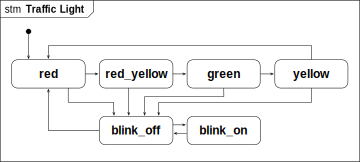
\includegraphics[width=\linewidth]{/Users/kraemer/Dropbox/Teaching/TTM4115/website 2020/cached/traffic-light-4.pdf}%
\label{default}
\end{center}
\end{figure}
Noice the detailed elements in this diagram:

\begin{itemize}
\tightlist
\item
  The frame has a five-cornered compartment at the top, showing the name
  of the state machine, prefixed with the keyword \texttt{stm}.
\item
  The states are shown as rounded rectangles. The state names are shown
  in bold text. As a naming convention, we only use lowercase letters,
  numbers, and underscores for state machine names, similar to rules for
  variable names in programming languages.
\item
  The start of the state machine is shown by a compact black dot. This
  is also a state, called the \emph{initial state}. Once the state
  machine is activated, it leaves this initial state.
\end{itemize}

\hypertarget{states}{%
\subsection{States}\label{states}}

State symbols with the same name refer to the same state. This means, we
can use a copy of the state symbol to make our layout easier, without
changing what we actually mean by the diagram. For instance, we can
remove the long arrow from state \texttt{yellow} to state \texttt{red}
just by having another copy of the symbol for state \texttt{red}:

\begin{figure}[htbp]
\begin{center}
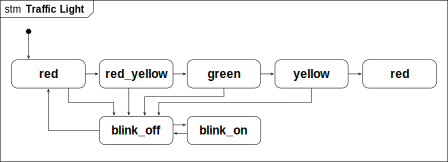
\includegraphics[width=\linewidth]{/Users/kraemer/Dropbox/Teaching/TTM4115/website 2020/cached/traffic-light-5.pdf}%
\label{default}
\end{center}
\end{figure}
The diagram describes exactly the same behavior. Both state symbols for
the state \texttt{red} refer to the same state, so our traffic light
still has the same number of states, just its layout changed. In this
simple state machine this doesn't really matter, but this can help you
to create better layouts once state machines become larger.

\textbf{State Names:} Selecting good names for states can help making
state machine easier to understand, especially when the states map to
phases of the thing we want to model, like \emph{on} and \emph{off} for
a lamp, or \emph{open} and \emph{close} for a lock. However, sometimes
there is no obvious good name. In such cases, I recommend to use state
names like \texttt{s0}, \texttt{s1},\ldots, which can make life easier.
You always have the possibility to attach a note to a state and explain
what it means.

Pay attention to the state symbol. It's a rectangle with some rounded
corners, nothing else!

\begin{figure}[htbp]
\begin{center}
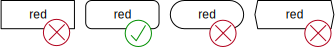
\includegraphics[width=\linewidth]{/Users/kraemer/Dropbox/Teaching/TTM4115/website 2020/cached/state-shapes.pdf}%
\label{default}
\end{center}
\end{figure}
\hypertarget{transitions}{%
\subsection{Transitions}\label{transitions}}

The arrows between the states are called \textbf{transitions}. We have
said above that the state machine is at any point in time in exactly one
of its states. It is not in two or more of them at the same time, and it
is never somewhere in between. Conceptually, this means that a state
machine switches from one state to another \textbf{within no time at
all}, meaning that \textbf{transitions take no time}. This sounds
magical, but we will come back to this.

So far, we have not yet talked about \emph{when} a transition happens,
this means, what \textbf{triggers} a transition. We have, for example,
not described \emph{when} the traffic light switches from \texttt{red}
to \texttt{red\_yellow}. There are three types of events that can
trigger transitions in a state machine:

\begin{itemize}
\tightlist
\item
  The state machine is started, then its \textbf{transition from the
  initial state} is triggered. This happens when the component or code
  surrounding the machine is started and then starts up the machine, for
  instance when we boot our firmware and the software starts running.
\item
  The state machine observes the \textbf{expiration of a timer}. Timers
  are managed by the machine itself, and we will learn how timers can be
  started and stopped later.
\item
  The state machine \textbf{receives a message.} State machines can
  receive messages from other parts of the system, which can be code,
  drivers, interrupts or communication modules, or other state machines.
\end{itemize}

A transition must have exactly one trigger. Without one, it would never
be started at all. For simplicity, we also don't allow more than one
trigger. A trigger is declared using a label on the arrow, followed by a
\texttt{/}. This means that you should have a trigger label at all
transitions, with the only exception being transitions starting at
initial states, because their trigger is implicitly the start of the
entire machine.

\hypertarget{actions}{%
\subsection{Actions}\label{actions}}

Let's have a look at a blinking light that you find often at the entry
of tunnels. The light blinks with two lamps to indicate that the tunnel
is closed. The blinking happens so that either the left lamp or the
right lamp are on, and they switch every second.

\begin{figure}[htbp]
\begin{center}
\includegraphics[width=\linewidth]{../figures/statemachines/tunnel.jpg}%
\label{default}
\end{center}
\end{figure}
From our experience with the more complex traffic light, this should be
an easy state machine to write down. It has two states, \texttt{left}and
\texttt{right}, corresponding to one of the lamps being switched on. We
also added labels to some of the transitions. They describe that the
state machine switches from state \texttt{left} to state \texttt{right}
triggered by an event \texttt{t1}. This is a timer. It switches back
with a timer \texttt{t2}. The detailed timer operations are not yet
visible, we come later to that. In this blinking light we also show how
to switch it off. This happens by an event called \texttt{off}, and it
can happen in any of the two states.

\begin{figure}[htbp]
\begin{center}
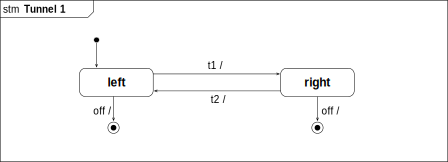
\includegraphics[width=\linewidth]{/Users/kraemer/Dropbox/Teaching/TTM4115/website 2020/cached/tunnel-1.pdf}%
\label{default}
\end{center}
\end{figure}
Now we also want to specify the actions to switch the individual lamps
on and off. We assume that we have for this the actions
\texttt{left\_on()}, \texttt{left\_off()}, and \texttt{right\_on()},
\texttt{right\_off()}. We already use Python syntax for these actions.
In our state machine diagram we can use these actions and add them to
the transitions.

The actions are also called an \textbf{effect} of the transition, and
happen at the same instant the transition is executed, that means, when
we switch states. The effects are written behind the \texttt{/} of the
transition label.

\begin{itemize}
\tightlist
\item
  The state machine runs action \texttt{left\_on()} when it starts, as
  declared by the initial transition.
\item
  When the machine switches from state \texttt{left} to \texttt{right},
  it runs actions \texttt{left\_off()} and \texttt{right\_on()},
  separated with a \texttt{;}.
\item
  When the machine switches from state \texttt{right} to \texttt{left},
  it runs actions \texttt{right\_off()} and \texttt{left\_on()},
  separated with a \texttt{;}.
\item
  When the blinking light switches off and moves into the final state,
  we run actions \texttt{left\_off()} or \texttt{right\_off()},
  depending on in which of the two states we are.
\end{itemize}

\begin{figure}[htbp]
\begin{center}
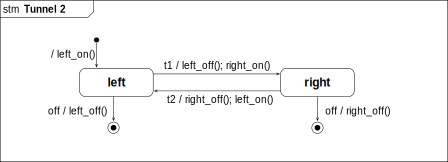
\includegraphics[width=\linewidth]{/Users/kraemer/Dropbox/Teaching/TTM4115/website 2020/cached/tunnel-2.pdf}%
\label{default}
\end{center}
\end{figure}
Another way to execute actions is to add them to a state, and run them
when we enter or exit the state. For some problems, such as the blinking
light, this makes the diagram much nicer. Have a look at the
functionally equivalent diagram:

\begin{figure}[htbp]
\begin{center}
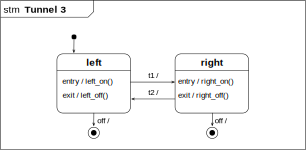
\includegraphics[width=\linewidth]{/Users/kraemer/Dropbox/Teaching/TTM4115/website 2020/cached/tunnel-3.pdf}%
\label{default}
\end{center}
\end{figure}
Here we have drawn the state symbol with a compartment and add entry and
exit actions to it. Actions that are preceded with the prefix
\texttt{entry/} are executed when the state machine enters the state,
and actions preceded with the prefix \texttt{exit/} run when the machine
exits the state. In the example this cleans up the entire diagram, since
we also can remove the actions from the initial transition and the
transitions that target the final states. When we before had to add
actions to all transitions entering or exiting a state, it is now enough
to only declare them once within the state.

You can list as many entry and exit actions for a state as you need,
just add a new line with the prefix \texttt{entry/} or \texttt{exit/}
for each of them. And of course, it looks nice when you list all entry
actions above the exit actions. We also assume that they are executed in
the way they are sorted, that means when we enter a state then the entry
actions are executed in the order they are written, and the same for the
exit actions when we exit the state.

\begin{figure}[htbp]
\begin{center}
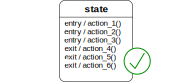
\includegraphics[width=\linewidth]{/Users/kraemer/Dropbox/Teaching/TTM4115/website 2020/cached/many-actions.pdf}%
\caption{Several entry and exit actions are possible.}
\label{default}
\end{center}
\end{figure}
\textbf{Mind the Slash!} The slash on the transition labels separates
the triggers from the actions.

\begin{itemize}
\tightlist
\item
  For initial transitions (the ones originating at an initial state)
  that do not have an action, the label is empty.
\item
  For initial transitions with actions, we add the slash before the
  actions: \texttt{/a1();\ a2()}
\item
  For actions that do not start at the initial state, they need to
  declare exactly one trigger, followed by the slash. Optionally, they
  can declare actions as they need. For instance \texttt{t1/} or
  \texttt{t1/a1();\ a2()}.
\end{itemize}

\hypertarget{timers}{%
\subsection{Timers}\label{timers}}

The expiration of a timer can trigger a transition. By convention, we
name timers with a prefix \texttt{t}, like for example \texttt{t0}. To
declare that a transition is triggered by a timer, we simply write the
name of the timer in the beginning of the transition label.

State machines manage timers on their own, wich also means that timers
can only be started as part of an action within the same state machine.
As we anticipate already our implementation in Python, we use the
following syntax for controlling timers:

\begin{itemize}
\tightlist
\item
  \texttt{start(t1,\ 1000)} starts a timer with name \texttt{t1} that
  will expire after 1000 milliseconds. If we invoke this action again
  while the timer is active and has not yet expired yet, the countdown
  will again start from the beginning, i.e., we expect the timeout 1000
  milliseconds from the last call of \texttt{start(t1,\ 1000)}.
\item
  \texttt{stop(t1)} stops a timer, so that a timeout will not happen in
  the future. In case this action is called but \texttt{t1} already
  expired or was never started before, nothing happens.
\end{itemize}

\hypertarget{spaghetti-timer-example}{%
\subsubsection{Spaghetti Timer Example}\label{spaghetti-timer-example}}

Imagine we want to describe the behavior of a simple spaghetti timer.
This timer expires after 10 minutes and then beeps for 3 seconds. We can
do this with the state machine below.

\begin{figure}[htbp]
\begin{center}
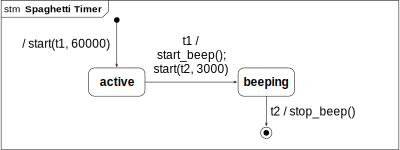
\includegraphics[width=\linewidth]{/Users/kraemer/Dropbox/Teaching/TTM4115/website 2020/cached/spaghetti-1.pdf}%
\caption{Simple timer that beeps for 3 seconds after 10 minutes are over.}
\label{default}
\end{center}
\end{figure}
Using entry and exit action on the states, we can also write this one in
a more compact form.

\begin{figure}[htbp]
\begin{center}
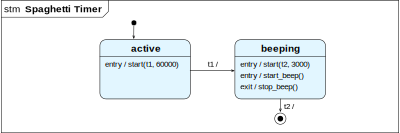
\includegraphics[width=\linewidth]{/Users/kraemer/Dropbox/Teaching/TTM4115/website 2020/cached/spaghetti-2.pdf}%
\caption{Functionally identical timer, but with entry and exit actions on the
state.}
\label{default}
\end{center}
\end{figure}
\textbf{Exercise:} Simulate both of these state machines in you head or
on paper by going through all the states, starting with the initial
state. Verify that these two versions really are functionally
equivalent.

\hypertarget{internal-transitions}{%
\subsection{Internal Transitions}\label{internal-transitions}}

You have seen that we can declare entry and exit actions within a state
symbol, which lets us in some cases describe more compact state
machines. Another thing we can declare within a state is an
\textbf{internal transition}. The internal transition has a label like
normal transitions, \texttt{trigger/actions} but is written inside the
state symbol, between the entry and exit actions.

\begin{figure}[htbp]
\begin{center}
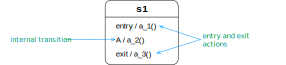
\includegraphics[width=\linewidth]{/Users/kraemer/Dropbox/Teaching/TTM4115/website 2020/cached/internal-transition.pdf}%
\caption{Declaration of an internal transition, triggered by event A.}
\label{default}
\end{center}
\end{figure}
The state \emph{s1} above declares an internal transition
\texttt{A/a\_2()}. It is triggered when the event \texttt{A} is
happening. When that happens, action \texttt{a\_2()} is executed.
Because it is an internal transition, the entry and exit actions are
\textbf{not} executed. Also, because the state stays the same, we can
react many times to the event \texttt{A}. Whenever it occurs and we are
in state \emph{s1}, action \texttt{a\_2()} will be executed.

\textbf{Note:} When you look at the entry and exit actions, you see that
they almost look the same as an internal transition. And the notation is
quite consistent, because the prefix \emph{entry} and \emph{exit} before
the \texttt{/} really do describe when the action behind the dash is
executed. But these are not transitions, just declarations of entry and
exit actions.

\hypertarget{choice-states}{%
\subsection{Choice States}\label{choice-states}}

In some cases, we want to have a choice in which state a transition
should switch, based on conditions in data. As an example, let's look at
the incomplete state machine below. It describes a part of a controller
for a heater. In state \texttt{heater\_on} we wait for 1 second for
timer \texttt{t}, which triggers the transition towards the choice
state. This choice state has two alternative branches, distinguished by
two guards, in rectangular brackets. Think of them as an if-statement in
a programming language. if the temperature is okay, we switch into state
\texttt{heater\_off}. If not, we take the else-branch and restart the
timer, to check again in another 1000 milliseconds.

\begin{figure}[htbp]
\begin{center}
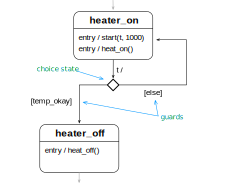
\includegraphics[width=\linewidth]{/Users/kraemer/Dropbox/Teaching/TTM4115/website 2020/cached/heater.pdf}%
\caption{Part of a temperature controller, using a choice state with guards to
make a decision.}
\label{default}
\end{center}
\end{figure}
Don't worry too much about what to write into the guard for now. This
will get much clearer once we implement state machines in Python, where
we implement the entire choice state with a Python if-statement.

A choice state can have many outgoing branches. One of them must have a
guard that is true, otherwise the state machine would be blocked. I
therefore recommend to have an else-branch, which is true whenever none
of the other branches is true.

By the way: There is one imperfection with this machine: When the
temperature is not okay yet, we re-enter the state \texttt{heater\_on},
which means that we execute entry action \texttt{heat\_on()} again. We
assume here that it is programmed in such a way that this doesn't
matter. An alternative is to add the action to both incoming transitions
of state \texttt{heater\_on}.

\hypertarget{transitions-revisited}{%
\subsection{Transitions, Revisited}\label{transitions-revisited}}

Now you have seen many kinds of transitions, and we can summarize all
the different terms for them. Knowing these terms makes talking about
state machines much easier when you design one together with other
engineers. So we have the following transitions:

\begin{itemize}
\tightlist
\item
  An \textbf{initial transition} originates at an initial state. It does
  not declare a trigger, since it is executed immediately when the state
  machine starts.
\item
  A \textbf{self-transition} is simply a transition that starts and ends
  in the same state.
\item
  An \textbf{internal transition} is a transition that starts and ends
  in the same state, but which does not invoke any of the state's entry
  and exit actions.
\item
  An \textbf{external transition} is the type of transition that is
  \emph{not an internal transition}. That means, a ``normal'' transition
  form one state to another, a self-transition, or an initial
  transition.
\end{itemize}

\hypertarget{transition-labels}{%
\subsubsection{Transition Labels}\label{transition-labels}}

We have seen now all the types of elements that we can add into the
label of a transition. This summarizes information from above, and you
can read it as a repetition:

\begin{itemize}
\tightlist
\item
  \textbf{Guards:} Transitions originating in a choice state must have
  them.
\item
  \textbf{Triggers:} All transitions originating in a normal state must
  declare a trigger, which is either the reception of a message or the
  expiration of a timer. Pseudostates like initial states or choice
  states are transient, and the outgoing transitions therefore do not
  declare a trigger.
\item
  \textbf{Effects:} Any transition can declare any number of action that
  it executes. Several actions are separated by a semicolon.
\item
  \textbf{Dash (/):} The dash separates triggers from actions. When a
  transition has either of them, we write the dash.
\end{itemize}

\hypertarget{states-revisited}{%
\subsection{States, Revisited}\label{states-revisited}}

Let's also have a look at all the different states we have seen until
now, and repeat some properties:

\begin{itemize}
\tightlist
\item
  Initial states and choice states are called \textbf{pseudo states},
  because they are not really states in the sense that we wait in them.
  They are transient states, meaning that the state machine is only
  going through them, but never waits in them. For that reason,
  transition originating at initial or choice states do not declare a
  trigger.
\item
  At any time, a state machine is in exactly one of its states. We
  assume that transitions execute in no time, so we never find a state
  machine like ``waiting'' within a transition. Waiting only happens
  within states.
\item
  State symbols with the same name refer to the same state.
\item
  State symbols are a compact rounded rectangle, and optionally contain
  a compartment where we can declare entry actions, exit actions and
  internal transitions.
\end{itemize}

\hypertarget{sending-messages}{%
\subsection{Sending Messages}\label{sending-messages}}

State machines can send and receive messages. You may think that this is
useful for implementing communication, like via TCP/IP or other
protocols. But the motivation is actually different. By sending
messages, we can couple state machines with each other, and handle
certain complex behavior easier. We can for example solve a problem with
two state machines that execute parallel to each other, and just
synchronize with each other every now and then via passing messages
between each other.

To send a message, we use the action
\texttt{send(\textquotesingle{}A\textquotesingle{},\ \textquotesingle{}stm1\textquotesingle{})},
where the first argument is the name of the message, and the second the
name of the state machine we want to send the message to.

Messages are received simply by declaring them as triggers.

\textbf{Example:} We want to extend our spaghetti timer from above. The
new timer should blink a light while it is active. Have a look at the
two coupled state machines below. The one at the top has the control of
the 10 minute timer, and waits until a user activates it via message
\texttt{start}. This message can come from a user interface, which we
don't show here. Once this message arrives, the machine switches into
state \texttt{active}, which declares the entry actions that start the
10 minute countdown timer \texttt{t1}, and another entry action that
sends message \texttt{on} to the machine to the right. This machine
takes only care of the blinking light, 1 sec on and 1 sec off.

\begin{figure}[htbp]
\begin{center}
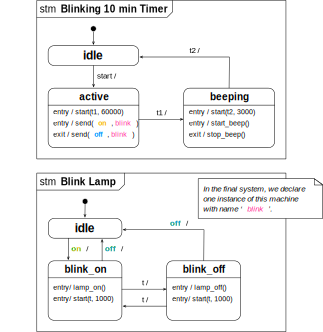
\includegraphics[width=\linewidth]{/Users/kraemer/Dropbox/Teaching/TTM4115/website 2020/cached/blinking-timer.pdf}%
\label{default}
\end{center}
\end{figure}
Now we \emph{could} build a single state machine for it, which handles
the 10 minutes timeout and the 1 sec blinking at the same time. But
imagine that the timer has more complicated functions, like restarting,
pausing, or it would be an entire different application with more
functions to integrate. Then it comes in very handy that you can start
and stop a sub-function such as blinking a light just by sending
messages to it from another machine.

\hypertarget{traces}{%
\subsection{Traces}\label{traces}}

Once you get more experienced with state machines, you will be able to
simulate them in your head, just by figuring out the sequences in which
the different events may happen. Since at any time, more than one event
could happen, the same state machine could create many different
sequences of events, also called \textbf{traces}. When you will design
state machines, it means to get control over all of these traces, so
that in the end, any possible behavior (that means, any possible trace
of events) is okay for the system. State machines hence describe
\textbf{complete behavior}. (We will later see how another diagram type,
interactions, describe usually only partial behavior.) For state
machines, this means that what they don't describe, they can't do.

By looking at a state machine, we can write down possible sequences of
events. Lets just write down \textbf{one} trace of events that can
happen when we activate the spaghetti timer. We just write down the
events regarding the main machine \textbf{Blinking 10 min Timer}, and do
so by listing the sequence of all triggers and actions as they happen:

\begin{itemize}
\tightlist
\item
  initial transition
\item
  message start received
\item
  entry action \texttt{start(t1,\ 1000)} in state \texttt{active}
\item
  entry action \texttt{send(on,\ blink)} in state \texttt{active}
\item
  timer \texttt{t1} expires
\item
  exit action \texttt{send(off,\ blink)} in state \texttt{active}
\item
  entry action \texttt{start(t2,\ 3000)} in state \texttt{beeping}
\item
  entry action \texttt{start\_beep()} in state \texttt{beeping}
\item
  timer \texttt{t2} expires
\item
  exit action \texttt{stop\_beep()} in state \texttt{beeping}
\end{itemize}

Here there is actually only a single behavior, because we go through the
states based on the timeouts of the two timers \texttt{t1}and
\texttt{t2}. A more realistic timers would also describe behavior where
we could abort it, which would be another trace.

\textbf{Exercise:} Put your finger on the state machine \textbf{Blinking
10 min Timer} and follow through the trace above. Note that the event
that timer \texttt{t1} expires happens \emph{before} the exit action
\texttt{send(off,\ blink)} in state \texttt{active} happens. This is
because the timer expiration of \texttt{t1} \emph{causes} this
transition and action. (Some students find that not intuitive, since the
timer \texttt{t1} is graphically outside of the state, and somehow looks
graphically to happen ``later'' in time.)

\hypertarget{state-transition-tables}{%
\subsection{State-Transition Tables}\label{state-transition-tables}}

So far, we used diagrams to write down our state machine. Instead we can
also use a table that lists all the transitions. This will be the basis
for implementing state machines in Python. There's not much more to say
about this table, other than that it offers another way of looking at a
state machine, and understand them systematically. Below you see again
the state machine for the tunnel light, and the table that describes the
same behavior. Check if you understand what each row means, and how it
corresponds line by line to the diagram.

\begin{figure}[htbp]
\begin{center}
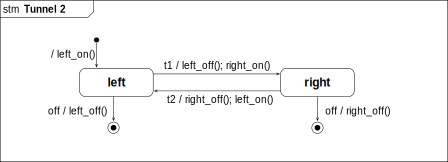
\includegraphics[width=\linewidth]{/Users/kraemer/Dropbox/Teaching/TTM4115/website 2020/cached/tunnel-2.pdf}%
\label{default}
\end{center}
\end{figure}
\begin{table*}[t]
\begin{tabulary}{\textwidth}{LLLL}
\toprule
Source State
&Trigger
&Actions
&Target State
\\
initial
&-
&left\_on()
&left
\\
left
&t1
&left\_off(); right\_on()
&right
\\
left
&off
&left\_off()
&final
\\
right
&t2
&right\_off(); left\_on()
&left
\\
right
&off
&right\_off()
&final
\\
\bottomrule
\end{tabulary}
\end{table*}



\hypertarget{a-physical-state-machine-model}{%
\subsection{A Physical State Machine
Model}\label{a-physical-state-machine-model}}

State machines are implemented in code and executed by a computer. To
understand how a state machine works, you can also think of them as a
physical machine, which executes almost like a mechanical clockwork. The
figure below illustrates such a machine.

\begin{figure}[htbp]
\begin{center}
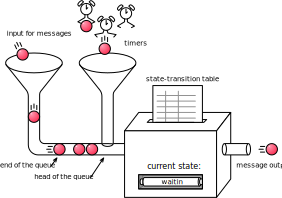
\includegraphics[width=\linewidth]{/Users/kraemer/Dropbox/Teaching/TTM4115/website 2020/cached/state-machine-machine.pdf}%
\caption{An imaginary machine that illustrates how a state machine works.}
\label{default}
\end{center}
\end{figure}
The state machine has an input queue for messages sent by other parts of
the system. These may be other state machines within the same computing
node, state machines from other nodes, or other parts of programs that
send messages.

All messages arrive and are sorted in a first-in, first-out (or short
FIFO) order.

The state machine also manages a set of timers. The state machine starts
these timers as part of its behaviour. When a timer expires, it places
an event in the same event queue as the one for incoming messages. Timer
expiration events are placed at the front of the queue, since an event
from a timer should be processed as close to its actual expiration time
as possible.

The state machine interprets the state machine diagram. The diagram can
be represented as a state-transition table, as we have seen above. In
this table is written down in which current state of the state machine
an event has which effect. The effect means the behaviour the state
machine is executing. This includes to start and stop timers, run
operations, and moving the state machine into its next state. The state
machine can also keep track of other data by using variables. This is
why this type of state machine is also called \emph{extended} finite
state machine.

\hypertarget{queue-semantics}{%
\subsubsection{Queue Semantics}\label{queue-semantics}}

To understand how a state machine executes, it is important to
understand how the input queue works.

\begin{itemize}
\tightlist
\item
  Messages arriving at the input of the state machine are placed
  \textbf{at the end} of the queue.
\item
  Time events are placed at the \textbf{front of the queue} when the
  corresponding timer expires.
\item
  States can defer events. (See below.)
\item
  Events that are not consumed or deferred are simply discarded, that
  means thrown away.
\end{itemize}

\textbf{Discarding events:} When the state machine is in a state that
does not declare a transition that is triggered by the event at the head
of the queue, the event is taken from the queue and discarded, that
means thrown away.

\begin{figure}[htbp]
\begin{center}
\includegraphics[width=\linewidth]{../figures/statemachines/discard.png}%
\label{default}
\end{center}
\end{figure}
Look at the situation above. Assume that the state machine is currently
in state \texttt{s1}. When message \emph{b} arrives, it is not consumed,
since state \texttt{s1} only has a transition with a trigger \emph{a},
so the state machine only waits for \emph{a}. Message \emph{b} is
therefore discarded as soon as it arrives during state \emph{s1}. Note
that it is discarded even if it is consumed by the later state
\emph{s2}, which is not the current state.

Rule: make sure that all transitions are triggered by something-
--\textgreater{}

\hypertarget{thata-all.}{%
\section{That'a all.}\label{thata-all.}}

That was a lot of details about state machines, but that's all details
we need. The coming weeks you will gain more experience in the actual
engineering task, that is, decomposing a problem and designing a good
state machine for it. That won't be easy, but its a rewarding and useful
task that is also fun.

\hypertarget{state-machines}{%
\section{State Machines}\label{state-machines}}

Until now, you have learned about all the features that we need for
state machines, but you have not yet created one on your own.

Creating state machines is a valuable engineering task. While you do it,
you understand gradually more of your system and the task it should
solve. Usually, this is difficult in the beginning but gets easier as
you learn more. In some cases it may also happen that you need to start
over, because you have understood, for example, that it is easier to
model some behavior with a set of state machines instead of a single
one. This will get much better with some experience. But it is not
always difficult. Often, you manage to handle a problem after some
attempts and then you ``see'' that you have a good solution. In that
respect, state machines are very nice, because a problem, once modelled
properly, can be easily checked by executing the state machines.

During this and the following weeks, you get several opportunities to
design state machines. This is useful for you, since it allows you to
handle concurrency in systems correctly, which is useful no matter which
programming language or framework you will later use. Also, creating
state machines is a task that trains your generic skills as an engineer,
and many problems can be mapped to that of state machines.

\hypertarget{creating-high-quality-state-machines}{%
\section{Creating High-Quality State
Machines}\label{creating-high-quality-state-machines}}

State machines are precise artefacts that can take care of the detailed
behavior, so they are suitable for unambiguously define how a system
should work. In the end, you did a good job if you are able to map user
requirements to a set of consistent, high-quality state machines.

Check: With high quality, we mean here that:

\begin{itemize}
\tightlist
\item
  The state machine is syntactically correct.
\item
  The state machine describes behavior that makes sense and is clearly
  defined.
\item
  The state machine has a good layout that conveys how it works and
  helps the reader to understand it.
\item
  The state machine can be implemented in code.
\end{itemize}

How to get started, when your paper or editor is empty in the beginning?
It can actually be hard to create a state machine from scratch, also for
experts. Actually, I think I have never observed that even experts write
down a state machine correctly on the first attempt, because there is
always something that you forget. So, they key to creating a state
machine: \textbf{Don't even try to make it correct on the first attempt,
but approach it iteratively.} Sometimes it is a good idea to separate
the task of creating something from the test of validating it. Otherwise
it is easy to get stuck. So for state machines, we switch between
writing down a state machine and then checking it.

\begin{figure}[htbp]
\begin{center}
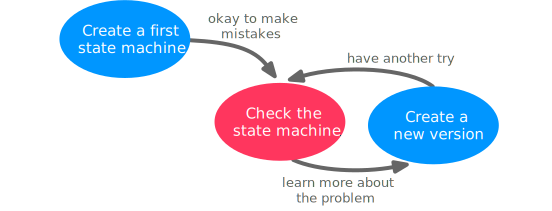
\includegraphics[width=\linewidth]{/Users/kraemer/Dropbox/Teaching/TTM4115/website 2020/cached/iterate.pdf}%
\caption{Switch between creating a state machine and checking it, so that you
don't get stuck.}
\label{default}
\end{center}
\end{figure}
\hypertarget{writing-down-a-state-machine}{%
\subsection{Writing Down a State
Machine}\label{writing-down-a-state-machine}}

To create down a state machine, don't ba afraid to just sketch a first
version. The following tips may help:

\begin{itemize}
\tightlist
\item
  \textbf{Start with pencil and paper}. Sometimes it is easier to
  explore design when you work alone, very focused and only with pencil
  and paper, where you can quickly sketch some states and transitions,
  without the pressure to make it work completely immediately. I have
  lots of experience in designing state machines. I still start with
  pencil and paper each time, before I go over to an electronic editor.
\item
  \textbf{Identify all triggering events}. Identify and write down all
  kinds of events that can trigger a transition in the state machine.
  Make a list of all incoming messages you may react to, and all timers
  that are necessary. Often these triggeres are determined by the
  problem to solve.
\item
  \textbf{Identify all actions.} Make a list of all actions that are
  used by your state machine to achieve its purpose. In this course, we
  use actions that we can use in Python.
\item
  \textbf{Identify any messages to send.} If the state machinen
  communicates with another one, you should list all messages it may
  send to the other machine, which you can treat just like an action.
  Note that all messages to receive is already included in th elist of
  triggers above.
\item
  \textbf{Introduce one state after the other}, and try to map states to
  states of whatever your state machine describes. Sometimes, some
  states are quite obvious, like the states of a lamp, which are
  \texttt{on} and \texttt{off}. Sometimes, you disciver that your
  problem has actually more states than you initially thought. For
  example can an electronic door lock have more than the obvious states
  \texttt{locked} and \texttt{unlocked}. The lock may be
  \texttt{engaged} meaning that it can be potentially opened, but if the
  user does not open it, it goes back into its \texttt{locked} state.
  Working with the problem will reveal this.
\item
  \textbf{Identify a default state}. For some problems, it may help to
  think of a default state that the state machine should be in. It may
  then be easier to explore the other states based on this. For example,
  think of a doorlock. It may be easier to design a state machine for it
  when you start thinking of it being locked first when the system
  starts, and then think what should happen to open it.\\
\item
  \textbf{Explore the problem}. Most likely, you will explore the
  problem and find out that you haven't understood everything, or that
  there are details that you have overlooked in the beginning. Be aware
  of what you learn, and how you can represent it with states and
  transitions. he state machine challenges you to learn more about the
  system.
\item
  \textbf{Start fresh}. When you get completely stuck, throw your sketch
  away and start fresh.
\end{itemize}

\begin{figure}[htbp]
\begin{center}
\includegraphics[width=\linewidth]{../figures/statemachines/sketching.jpg}%
\caption{It's a good idea to start with a sketch using paper and pencil and start
simple.}
\label{default}
\end{center}
\end{figure}
\hypertarget{checking-state-machines}{%
\subsection{Checking State Machines}\label{checking-state-machines}}

Once you have a state machine, even a partial one, you can check if it
can actually work.

For each of its \textbf{states}, you should check:

\begin{itemize}
\tightlist
\item
  \textbf{Are all states reachable?} This means, can you start at the
  initial state and from there reach any of the other states by
  following a sequence of events? Or are there some states that you can
  never reach? Obviously, that must be a mistake, because if these
  states are not reachable, what's the point in having them? Din the
  missing transitions towards these states and try again.
\item
  \textbf{Is there a deadlock?} This means, is there a state from which
  you cannot find out way out, for instance to a final state that
  terminates the machine? If there is a state that you cannot leave
  anymore, is that intended by the application?
\item
  \textbf{Are all possible events handled?} In each state, did you think
  of any events that may arrive? Remember, that events arriving at the
  head of the queue and that are not exoected in the form of triggers
  are discarded, that means, thrown away. Check if you have missed some!
\end{itemize}

For each \textbf{transition} you should check:

\begin{itemize}
\tightlist
\item
  \textbf{Does every transition have a triggering event?} This means
  that every transition must declare a trigger in the form of a message
  reception, a timer expiration, unless it is an intial transition or
  following a choice pseudo state.
\item
  \textbf{Do transitions with choice states block?} Decisions must not
  block, which means that one of the outgoing branches of a choice state
  must have a guard that is \texttt{True}. The safest way to achieve
  this is by letting one of the outoing branches have an \texttt{else}
  branch.
\end{itemize}

For each \textbf{timer} you should check:

\begin{itemize}
\tightlist
\item
  \textbf{Are timers properly started?} All timers must be started by
  the machine itself, so a timer that is not started will never expire
  and is hence not useful. Find a proper place to start it, either as
  part of a transition effect or as entry or exit actions, just like
  other actions.
\item
  \textbf{Are timer expirations handled?} Check what happens when a
  started timer expires. If a timeout happens in a state that does not
  decløare an outgoing transition triggered by it, it is simply ignored.
  This may be okay in your machine (because something else happended and
  you don't need the timer anymore), but it can also be the sign of an
  error.
\end{itemize}

These are the rules that you can check even without knowing exactly what
the application should do, just by looking at the state machines. These
are generic rules, independent of a specific application, and if they
don't hold, it is very likely that you do have a problem. But then there
are also errors that have to do with your specific \textbf{application.}
This can be a bit harder to find out. You need to simulate the state
machines using your fingers and go through it state by state and event
by event. When the problem is not too big, this is possible. Next week,
once we implement state machines in Python, you will also be able to
build functioning prototypes, which you can use and test to see how the
final state machine behaves.

\hypertarget{getting-started-bus-stop}{%
\section{Getting Started: Bus Stop}\label{getting-started-bus-stop}}

You should build the state machine for a bus stop signal light. It is
intended for bus stops where busses only halt when there are passengers,
and which are located so that it is difficult for a bus driver to see
passengers when they approach. It may also be that they need to get off
a larger road, but can stay on that road if there are not passengers.
The solution is a signal light that passengers can activate at the buss
top and which is better visible for the approaching bus.

\begin{figure}[htbp]
\begin{center}
\includegraphics[width=\linewidth]{../figures/statemachines/bus-1.png}%
\caption{Sketch of the bus stop.}
\label{default}
\end{center}
\end{figure}
Here are the detailed functional requirements:

\begin{itemize}
\tightlist
\item
  Passengers waiting at the bus stop can press a button, upon which the
  signal lamp switches on.
\item
  The bus driver can switch the light off via a radio message
  \texttt{bus}.
\item
  The light switches off 10 minutes after it was pressed, even if no bus
  came.
\item
  If a passenger presses the button and the light is already on, it
  stays on, but the 10 minutes timer starts again with 10 minutes.
\end{itemize}

Use the following elements:

\begin{itemize}
\tightlist
\item
  actions \texttt{lamp\_on()}, \texttt{lamp\_off()},
  \texttt{start\_timer(\textquotesingle{}t\textquotesingle{},\ 600000)}
\item
  triggers \texttt{switch}, \texttt{bus}, \texttt{t}
\item
  states \texttt{on}, \texttt{off}, and an initial state
\end{itemize}

You can ignore for now that the system may be switched off, so you need
no final state.

\hypertarget{create-a-state-machine-individually}{%
\subsection{Create a State Machine,
Individually}\label{create-a-state-machine-individually}}

\begin{itemize}
\tightlist
\item
  Use some time to find a first solution each one on your own.
\item
  Use pencil and paper.
\end{itemize}

\hypertarget{create-a-state-machine-together}{%
\subsection{Create a State Machine,
Together}\label{create-a-state-machine-together}}

\begin{itemize}
\tightlist
\item
  Compare your solutions, one at a time.
\item
  Starting again with an empty screen, whiteboard or paper, design the
  state machine once again, together.
\item
  Play through this simple scenario, and correct your state machine if
  necessary.
\end{itemize}

\hypertarget{solution}{%
\subsection{Solution}\label{solution}}

\begin{itemize}
\tightlist
\item
  Once you are happy with your solution, have a look at
  \href{files/bus-stop.pdf}{my solution}.
\item
  Compare the solutions in detail.
\item
  If you find that my solution has any flaws, please discuss on MS
  Teams!
\item
  Prepare a document where you show your solution and mine side-by-side,
  and compare.
\item
  Reflect about your process towards this machine.

  \begin{itemize}
  \tightlist
  \item
    What did you get right immediately?
  \item
    What was difficult?
  \item
    Were there misunderstandings?
  \end{itemize}
\end{itemize}

\hypertarget{kitchen-timer}{%
\section{Kitchen Timer}\label{kitchen-timer}}

You should build the state machine for the following device:



\includegraphics[width=\linewidth]{../cached/aaaa66.jpg}
\url{https://youtu.be/Gnjg16f6DhY}
It's a kitchen timer. It has 4 LEDs and a button. When the button is
pressed, the first LED is switched on, and the plug provides
electricity, for instance for a coffee machine. After 15 minutes, the
LED is switched off and the plug is turned off. Whenever the button is
pressed when an LED is already on, the next LED is switched on and time
timer is set to 30, 45, or 60 minutes, respectively. If all LEDs are on,
and the button is pressed, all LEDs and the plug are switched off.

You can ignore that the LED of the segment that is currently active is
blinking, just assume it lights all the time.

Use the following actions:

\begin{itemize}
\tightlist
\item
  \texttt{start\_timer(\textquotesingle{}t\textquotesingle{},...\ )}
  This starts a timer with name \texttt{t}. The second argument is the
  time, given as seconds. If a timer is already active, the timer is
  simply restarted with the new, updated timeout.
\item
  \texttt{stop\_timer(\textquotesingle{}t\textquotesingle{})}. Stops a
  timer. If no such timer exists or has already timed out, nothing
  happens.
\item
  \texttt{set\_leds(1,\ 0,\ 0,\ 0)}. Control all of the four LEDs at the
  same time. \texttt{1} means on, \texttt{0} means off. Here, the first
  LED is switched on, the others are off.
\item
  \texttt{set\_power(True)} switches the power on (True) or off (False)
\end{itemize}

You can assume that whenever the button is pressed, the state machine
will receive a signal with the name \texttt{switch}.

\hypertarget{create-a-state-machine-individually}{%
\subsection{Create a State Machine,
Individually}\label{create-a-state-machine-individually}}

\begin{itemize}
\tightlist
\item
  Use some time to find a first solution each one on your own.
\item
  Use pencil and paper.
\end{itemize}

\hypertarget{create-a-state-machine-together}{%
\subsection{Create a State Machine,
Together}\label{create-a-state-machine-together}}

\begin{itemize}
\tightlist
\item
  Compare your solutions, one at a time.
\item
  Starting again with an empty screen, whiteboard or paper, design the
  state machine once again, together.
\item
  Play through this simple scenario, and correct your state machine if
  necessary.
\end{itemize}

\hypertarget{solution}{%
\subsection{Solution}\label{solution}}

\begin{itemize}
\tightlist
\item
  Once you are happy with your solution, have a look at
  \href{files/kitchen-timer.pdf}{my solution}.
\item
  Compare the solutions in detail.
\item
  If you find that my solution has any flaws, please discuss on MS
  Teams!
\item
  Prepare a document where you show your solution and mine side-by-side,
  and compare.
\item
  Reflect about your process towards this machine.

  \begin{itemize}
  \tightlist
  \item
    What did you get right immediately?
  \item
    What was difficult?
  \item
    Were there misunderstandings?
  \end{itemize}
\end{itemize}

\hypertarget{checklist}{%
\section{Checklist}\label{checklist}}

\hypertarget{blackboard}{%
\subsubsection{Blackboard}\label{blackboard}}

\begin{itemize}
\tightlist
\item
  Deliver the reflection over your solutions in comparison to the ones
  provided, both for the bus stop and the kitchen timer.
\end{itemize}

\hypertarget{ms-teams}{%
\subsubsection{MS Teams}\label{ms-teams}}

\begin{itemize}
\tightlist
\item
  Ask for feedback in general
\item
  Report any errors with the provided solution
\end{itemize}

\hypertarget{team-reflection-for-this-unit}{%
\subsubsection{Team Reflection for This
Unit}\label{team-reflection-for-this-unit}}

\begin{itemize}
\tightlist
\item
  Add another section to the team reflection document, just like last
  week.
\end{itemize}

\hypertarget{individual-reflection}{%
\subsubsection{Individual Reflection}\label{individual-reflection}}

\begin{itemize}
\tightlist
\item
  Fill out the individual reflection survey.
\item
  Copy the answers into a document that you maintain on your own.
\item
  Add any additional observations to your reflection diary.
\end{itemize}

\hypertarget{the-headphone-story}{%
\section{The Headphone Story}\label{the-headphone-story}}

This is an additional task if we have time left.

You work as a summer intern at a computer company during the spring of
2007. You get the task to develop a controller for a mysterious remote
control for some headphone stuff or so. Everyone is busy. A product
manager drops by, and tells you:

\begin{quote}
``The controller should translate button clicks into specific commands,
depending on how often the user clicks. A single click should generate
signal 'switch'. I think they use that for switching between playing and
pausing. A double click should send signal 'next'. And if the user
clicks three times in a row they need signal 'back'. That's all I know.
I have to go. Oh\ldots{} the guys from the X-department gave me a
diagram how it should be integrated. Here.''
\end{quote}

\begin{figure}[htbp]
\begin{center}
\includegraphics[width=\linewidth]{../figures/statemachines/headphones.png}%
\label{default}
\end{center}
\end{figure}
You are confused, but you manage to produce a decent state machine.

Create the state machine. You probably need some individual focus time
to try it out on a piece of paper before you sketch a solution in
Draw.io.

\clearpage\newpage
\chapter{Unit 2 — Interactions}
\hypertarget{interactions}{%
\section{Interactions}\label{interactions}}

State machines are suitable to show the behavior of a single component
at a time, and define its behavior in terms of states and transitions.
We have also seen that state machines are used to define a protocol, as
for instance TCP, by showing the behavior of each of the communication
partners. Sequence diagrams, on the other hand, are used to specify the
interactions between the components of a system. Interactions can happen
through method-, function- or operation-calls, or via signals. Sequence
diagrams specify therefor behavior by looking at the sequences of
interactions \emph{between} several components. These components can be
within the same computer or far away from each other. Some of the
components may not even be software.

\hypertarget{learning-goals}{%
\subsection{Learning Goals}\label{learning-goals}}

\textbf{goals:} After this week, you will be able to:

\begin{itemize}
\tightlist
\item
  Create syntactically valid sequence diagrams.
\item
  Validate sequence diagrams.
\item
  Reason about design choices using sequence diagrams.
\item
  Compare sequence diagrams based on their trace semantics.
\item
  Find and resolve implied scenarios.
\end{itemize}

An important difference to state machines is that sequence diagrams
usually do not model complete behaviors, but only show selected
scenarios that a developer wants to show. More on that later. Let's
first get some intuition on sequence diagrams.

\hypertarget{intuition-on-sequence-diagrams}{%
\section{Intuition on Sequence
Diagrams}\label{intuition-on-sequence-diagrams}}

Sequence diagrams are an effective and intuitive way to describe the
communication between several communicating partners. Have a look at the
following dialogue:

\begin{figure}[htbp]
\begin{center}
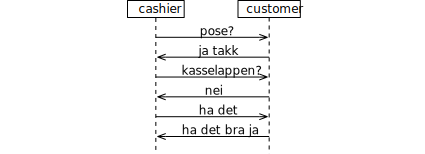
\includegraphics[width=\linewidth]{../figures/interactions/intuition.png}%
\caption{A sequence diagram showing a conversation.}
\label{default}
\end{center}
\end{figure}
That's pretty much how sequence diagrams work, they show messages
between participants. Each participant in a sequence diagram is
represented by a vertical line, called \emph{lifeline}. The horizontal
lines are messages. Time flows downwards, so that the messages make up a
conversation.

With this little knowledge, you can already understand most sequence
diagrams. What follows are refinements of this concept and additional
modeling elements so we can more precisely express how a software system
communicates. This is necessary to prevent misunderstandings between
developers and when we want to detect design flaws in our systems at an
early stage.

\hypertarget{participants-and-lifelines}{%
\subsection{Participants and
Lifelines}\label{participants-and-lifelines}}

Each participant in a sequence diagram is represented by a lifeline,
shown as dashed lines. It's okay to show them as solid lines, which may
sometimes be quicker when you make a sketch by hand. Lifelines are
always drawn parallel to each other, and follow a vertical orientation.
You will never see a sequence diagram with horizontal lifelines. If you
do, it's not a sequence diagram.

Lifelines can represent software concepts like components, modules,
objects or classes. They can also represent entities from reality, like
human users. The diagram below shows how a human user who presses a
button on a car key. The car key then sends a radio signal to the car,
which in turn confirms to the user by blinking the lights.

\begin{figure}[htbp]
\begin{center}
\includegraphics[width=\linewidth]{../figures/interactions/car-key.png}%
\label{default}
\end{center}
\end{figure}
The top of the lifeline shows a box that refers to what the participant
represents in this sequence diagram. The label in this box consists of
three parts: a role name, a selector, a class name.

\begin{verbatim}
role[selector]:Class
\end{verbatim}

Let's look at an example to understand the difference between these.
Below you see a sequence diagram of a home automation system. There are
several \textbf{roles}: \emph{sensor} and \emph{light}. The role name is
a name that refers to the participant's function within an interaction.
From the lifelines that represent sensors, the diagram shows that there
are two \textbf{classes} of sensors, \emph{TempSensor} and
\emph{HumiditySensor}. All of them act as sensors in the system (and
hence send signals with the name \emph{measurement}), which is why they
all share the same role. All components communicate with the central
unit. Here we have chosen to just give it a class name
\emph{HouseCentral}, since there is only one and we already know that we
want to have this class. An alternative would be to just give it a role
name, for instance \emph{central}. You can also see that the sensors
have different \textbf{selectors}, which here are strings that refer to
different rooms. They show that there can be many sensors (role
\emph{sensor} of the same class (for instance \emph{TempSensor}). Here,
room names make sense. Alternatives are numbers.

\begin{figure}[htbp]
\begin{center}
\includegraphics[width=\linewidth]{../figures/interactions/home-system.png}%
\label{default}
\end{center}
\end{figure}
A lifeline requires at least a role name or a class name. The selector
is optional. Note that the class name is always preceded by a colon
(``:''). Usually, role names are in lowercase letters, and class names
are written in CamelCase.

\hypertarget{messages}{%
\subsection{Messages}\label{messages}}

The horizontal arrows are called \textbf{messages}. They represent
either the transmission of a \textbf{signal}, or the \textbf{call of an
operation}.

\begin{itemize}
\item
  \textbf{Signals} represent information that is communicated
  asynchronously between objects. So far, all messages we have seen have
  referred to signals. They may refer to the physical touch of a button,
  a radio transmission, the signal of a light, a sound notification, or
  any other transmission of information. In the following, many of our
  signals will represent units of some specific protocol, like an MQTT
  or AMQP message. Signals are always asynchronous, and therefore use
  always the symbol for asynchronous messages, which is the solid line
  with an open arrowhead.
\item
  Alternatively, messages in sequence diagrams refer to
  \textbf{operation calls}. They correspond to functions, methods or
  operations in programming languages.
\end{itemize}

\begin{figure}[htbp]
\begin{center}
\includegraphics[width=\linewidth]{../figures/interactions/math-pow.png}%
\label{default}
\end{center}
\end{figure}
The figure above shows an example of a sequence diagram that shows the
communication between a Python main program \emph{main.py} that calls
the \emph{pow()} function of the \emph{math} module. As you can see,
this interaction is much more complicated than the one with the signals.
An operation call consists of two messages: the message that represents
the call of the operation, and another one that shows the return of the
operation. In the example, the operation also returns a result. The
messages are also drawn differently: The call message in this example is
a synchronous message, and therefore drawn with a filled arrowhead (as
opposed to the open arrowhead of the message that describes a signal).
The return message has an open arrowhead, but is painted with a dashed
line. Therefore, this is a synchronous function call, which represents
what the Python program actually does: The calling main.py is blocked
(not doing anything) while math.py is calculating the results and then
returns.

Sometimes the return message is left away, to reduce the visual clutter
of a diagram or just due to laziness. In this course, we don't do that
for didactic reasons, so that we can clearly distinguish the modeling of
signals from that of operation calls. If you use messages that represent
operation calls, always draw the return messages.

\begin{figure}[htbp]
\begin{center}
\includegraphics[width=\linewidth]{../figures/interactions/math-pow-3.png}%
\label{default}
\end{center}
\end{figure}
There are also situations where method calls in programming languages
are asynchronous. Then, the calling message is shown with the
asynchronous message symbol (the one with the open arrow head). In this
course, you will probably not use this and can forget about them.

\begin{figure}[htbp]
\begin{center}
\includegraphics[width=\linewidth]{../figures/interactions/math-pow-2.png}%
\label{default}
\end{center}
\end{figure}
The diagram above shows another element that is sometimes used:
\textbf{execution specifications}. These elements illustrate that a
participant is active. For instance, the main program is active, then
calling \emph{pow()}, which activates the math module until it returns.
In some cases, such an illustration is very helpful, for instance to
represent recursive method calls, or illustrate design patterns. In this
course, execution specifications are optional. In many situations it is
better to focus on the messages and get them right.

\hypertarget{creation-and-destruction}{%
\subsection{Creation and Destruction}\label{creation-and-destruction}}

In some cases, it is interesting to show that a participant in an
interaction is created or destroyed as part of the interaction. This is
shown by special messages. Creation messages target the head of the
lifeline that they create. Destruction messages target a lifeline that
is then terminated with a big termination symbol. Both messages are
shown as dashed lines with an open arrow. They can be labeled with the
\emph{create} and \emph{destroy} stereotypes. The example below shows
how the main program creates an object of type \emph{Socket} and then
destroys it again. Note that creation and destruction can be used
independently, and that they can be triggered by different participants
in the interaction. A lifeline can also terminate itself without a
destruction message.

\begin{figure}[htbp]
\begin{center}
\includegraphics[width=\linewidth]{../figures/interactions/create-destroy.png}%
\label{default}
\end{center}
\end{figure}
\hypertarget{what-do-sequence-diagrams-represent}{%
\section{What do Sequence Diagrams
Represent?}\label{what-do-sequence-diagrams-represent}}

Let's take a step back. You have seen that sequence diagrams can
represent a wide variety of interactions, and even include elements that
are not software. Within software, we can coarsely distinguish two
different focus areas covered by sequence diagrams:

\begin{itemize}
\item
  \textbf{Local interactions} \emph{within a program}, i.e., procedure,
  method or function calls.
\item
  \textbf{Distributed interactions} of a system that consists of
  \emph{several components}, each running some programs.
\end{itemize}

Note that both local and distributed interactions are represented with
several lifelines. In the local case, they represent different code
modules, like Java or Python classes or modules. Within both of these
interaction groups, you can use asynchronous signals or synchronous or
asynchronous operation calls. This means, there can be local signals,
and there are also distributed operation calls.

Sequence diagrams typically only show selected scenarios of the
interactions in a system, and do not give a complete picture. That means
they do not show all the possible exchanges of messages of a real
system, but focus only on a few but interesting ones. This may come as a
surprise. If we want to do a good specification job, don't we have to
study \emph{all} interaction scenarios? The problem is complexity.
Sequence diagrams can quickly grow, and a naïve attempt to cover all
scenarios just by writing them down results in specifications that
confuse rather than clarify. Important aspects of the model will drown
in too many details, and the value of modeling is lost. There are
several solutions to this dilemma:

\begin{itemize}
\item
  We will complement sequence diagrams with state machines, which give a
  complete picture, but on a local level only.
\item
  You will learn how to select the relevant and interesting interaction
  scenarios that deserve attention, and leave out those that are not
  relevant.
\item
  We will try to build interactions in such a way that the number of
  possibilities is reduced.
\end{itemize}

One way of making sequence diagrams more powerful and let a single
diagram express more than one scenario is by using combined fragments,
which we will look at in the next section.

\hypertarget{combined-fragments}{%
\section{Combined Fragments}\label{combined-fragments}}

Combined fragments allow you to express more behavioral details in
compact ways. Some of them look very much like programming statements,
which makes them intuitive to understand. However, it can also be a trap
to think of them too much as control statements, since they do not
handle operations, but entire scenarios. Rather, think of them as a way
to characterize interactions.

\hypertarget{alt}{%
\subsection{alt}\label{alt}}

The \textbf{alt} fragment specifies alternative scenarios. For instance,
a component may ask for access, and the access right may be granted or
not. We can show this in the sequence diagram \emph{Access} below:

\begin{figure}[htbp]
\begin{center}
\includegraphics[width=\linewidth]{../figures/interactions/alt.png}%
\label{default}
\end{center}
\end{figure}
The different compartments are alternatives to each other. There may be
any number of compartments, not only two. They are separated by a dashed
line. To describe in more detail, when a specific alternative is chosen,
the compartments can have an optional guard. This guard may refer to
some text or a variable.

\emph{Access} almost looks like an if-statement. And in fact, the access
control component may internally execute an if-statement. But the alt
fragment can be even more abstract, since it can describe alternative
scenarios, independent of how they are realized. The specification of
\emph{Timer} is therefore equally valid Do you see the difference? The
example shows that a timer can be started and then either be aborted or
it times out. This time the scenario is more subtle, the alternative is
not determined by a single component, but the overall timing of the
interaction.

\hypertarget{opt}{%
\subsection{opt}\label{opt}}

The \textbf{opt} fragment contains behavior that can happen or not. It
is similar to an alt fragment with two compartments, one of which is
empty. Like with the alt fragment, the opt fragment can have a guard.

\begin{figure}[htbp]
\begin{center}
\includegraphics[width=\linewidth]{../figures/interactions/opt-1.png}%
\label{default}
\end{center}
\end{figure}
\hypertarget{loop}{%
\subsection{loop}\label{loop}}

With the \textbf{loop} fragment, you can express that a behavior is
executed repeatedly. Below, you see the specification of an alarm clock
with a snooze function. Within the loop fragment, you see an alt
fragment, with different branches of the user either snoozing or
stopping the alarm. In case of stopping the alarm, there is also a break
fragment. This signals the escape out of the loop. You may also leave
unspecified how often the loop is executed.

\begin{figure}[htbp]
\begin{center}
\includegraphics[width=\linewidth]{../figures/interactions/loop-1.png}%
\label{default}
\end{center}
\end{figure}
\hypertarget{assert-and-neg}{%
\subsection{assert and neg}\label{assert-and-neg}}

In some cases, you want to assert that a certain interaction must
exactly occur as specified. For that, you can place it into an
\textbf{assert} fragment. The other way round, you may want to specify
\emph{negative} behavior, i.e., behavior that must not happen. Such
behavior can be places in a \textbf{neg} fragment.

\begin{figure}[htbp]
\begin{center}
\includegraphics[width=\linewidth]{../figures/interactions/assert-neg.png}%
\label{default}
\end{center}
\end{figure}
\hypertarget{ref}{%
\subsection{ref}\label{ref}}

With a \textbf{ref} fragment, you can refer from one sequence diagram to
another one. This makes diagrams easier to handle. It also allows to
reuse a sequence diagram and apply it at several places.

In the example below, we have another definition of the snooze feature
of an alarm clock. Here, we used the ref fragment that refers to the
sequence diagram itself and by that introduces some recursion. (The blue
arrow is just an illustration.) This is probably not a good example in
general, but it should work. Note that the outermost frame, labeled
``\textbf{sd} alarm'' encapsulates the entire sequence diagram.

\begin{figure}[htbp]
\begin{center}
\includegraphics[width=\linewidth]{../figures/interactions/ref-1.png}%
\label{default}
\end{center}
\end{figure}
\hypertarget{time-constraints}{%
\subsection{Time Constraints}\label{time-constraints}}

In some cases, you want to add time constraints to a specification, to
show \emph{when} an interaction occurs, or how long specific parts of it
may or should take. Have a look at the example below:

\begin{figure}[htbp]
\begin{center}
\includegraphics[width=\linewidth]{../figures/interactions/timing.png}%
\caption{From the UML@Class book.}
\label{default}
\end{center}
\end{figure}
It shows that the newsletter is sent at 12:00. Five time units later,
the student receives the confirmation. The diagram also specifies that
the signal \emph{inform} must be received within two hours.

\hypertarget{event-orderings-and-semantics}{%
\section{Event Orderings and
Semantics}\label{event-orderings-and-semantics}}

Let's have a closer look at the semantics of sequence diagrams, that is,
what they mean in detail. We do this by looking at the detailed events
that happen as part of an interaction. understanding in which order they
are supposed to happen, means to understand what the interaction really
means.

The passing of a message \textbf{A} consists of two events:

\begin{itemize}
\item
  The message is sent, written as \textbf{!A}.
\item
  The message is received, written as \textbf{?A}.
\end{itemize}

\textbf{Ordering Rule 1:} Because our universe seems to act causally,
\textbf{a message must be sent before it can be received}. For a message
A, the only sequence of events that it possible is
\(\langle !A, ?A \rangle\).

\textbf{Ordering Rule 2:} A second ordering rule is that of lifelines:
\textbf{Events along the \emph{same} lifeline are in a total order.}
Below, this means that lifeline Y receives signal A before it receives
B, \(\langle ?A, ?B \rangle\).

\begin{figure}[htbp]
\begin{center}
\includegraphics[width=\linewidth]{../figures/interactions/ordering-lifeline.png}%
\label{default}
\end{center}
\end{figure}
Now comes the part that may be less intuitive: Events on different
lifelines are \emph{not ordered}, even though they have distinct
y-coordinates. In the diagram below, the reception of A and the
reception of B are clearly at different y-coordinates. \emph{Visually},
A happens before B. But this is \emph{not} an order that the diagram
implies. Because these events are not related with each other, the
diagram does not tell if any of them happens before each other, despite
it may look like it.

\begin{figure}[htbp]
\begin{center}
\includegraphics[width=\linewidth]{../figures/interactions/ex-11.png}%
\caption{Despite the position on their respective lifelines, events ?A and ?B are
not in any order in this diagram.}
\label{default}
\end{center}
\end{figure}
For some, this non-ordering of events on different lifelines may not be
intuitive at the first glance. The following illustration may help you
to understand it: Imagine that the events along a lifeline are connected
to it by rings. The rings can move up and down along the lifeline, and
the message can get a different slope depending on the position on the
rings. Rings attached to the same lifeline can not pass each other.
Therefore, the diagrams below all look different, but imply the same
ordering among the events, irrespective of their absolute position on
the lifelines. What counts is that \(A\) is received before \(B\), and
this does not change in any of the diagrams.

\begin{figure}[htbp]
\begin{center}
\includegraphics[width=\linewidth]{../figures/interactions/ex-12.png}%
\label{default}
\end{center}
\end{figure}
The slope of messages is hence only a means of illustration. A
recommendation is to use horizontal messages where possible, and
messages with a downwards slope when you want to show that messages
cross each other. (That comes later.) Avoid messages with an upwards
slope.

The example below shows a sequence diagram with two messages, and four
distinct events:

\begin{figure}[htbp]
\begin{center}
\includegraphics[width=\linewidth]{../figures/interactions/ex-1.png}%
\label{default}
\end{center}
\end{figure}
Intuitively, we already know one sequence in which these events can
happen, that is, we know that \(\langle !A,?A,!B,?B \rangle\) is one
valid trace. However, it is not the only possible trace. To find the
other traces, we may start by writing down all possible different
combinations we can get from these events. With 4 events, we end up with
24 different traces:

\(\langle !A,?A,!B,?B \rangle, \langle !A,?A,?B,!B \rangle, \langle !A,!B,?A,?B \rangle, \langle !A,!B,?B,?A \rangle, \langle !A,?B,?A,!B \rangle, \langle !A,?B,!B,?A \rangle\)

\(\langle ?A,!A,!B,?B \rangle, \langle ?A,!A,?B,!B \rangle, \langle ?A,!B,!A,?B \rangle, \langle ?A,!B,?B,!A \rangle, \langle ?A,?B,!A,!B \rangle, \langle ?A,?B,!B,!A \rangle\)

\(\langle !B,!A,?A,?B \rangle, \langle !B,!A,?B,?A \rangle, \langle !B,?A,!A,?B \rangle, \langle !B,?A,?B,!A \rangle, \langle !B,?B,!A,?A \rangle, \langle !B,?B,?A,!A \rangle\)

\(\langle ?B,!A,?A,!B \rangle, \langle ?B,!A,!B,?A \rangle, \langle ?B,?A,!A,!B \rangle, \langle ?B,?A,!B,!A \rangle, \langle ?B,!B,!A,?A \rangle, \langle ?B,!B,?A,!A \rangle\)

Because of the ordering rules from above, not all of these traces are
possible. The sequence diagram \emph{Alpha} from above relates the four
events with each other.

\begin{itemize}
\item
  Because of message ordering, we know that only those traces are valid
  ones, in which a signal is sent before it is received. This means,
  \(!A\) must happen before \(?A\) and \(!B\) must happen before \(?B\).
\item
  Because of lifeline ordering, we also know that those traces, in which
  events do not follow the order of the lifeline, are invalid. This
  means \(!A\) must happen before \(!B\), and \(?A\) must happen before
  \(?B\).
\end{itemize}

\textbf{Exercise:} Can you find the traces that violate any of the two
ordering rules, and strike them out?

\hypertarget{co-regions}{%
\subsection{Co-Regions}\label{co-regions}}

The diagram \emph{Beta} below only covers the scenario that \(A\) is
received by \(Y\) before \(B\).

\begin{figure}[htbp]
\begin{center}
\includegraphics[width=\linewidth]{../figures/interactions/ex-2.png}%
\label{default}
\end{center}
\end{figure}
\textbf{Exercise:} Write down all the possible traces that the sequence
diagram \emph{Beta} allows.

In reality, it will be hard or impossible to ensure that this order is
maintained, especially since the diagram allows to send \(B\) first. For
a real and robust specification, we should handle such situations. One
way is to demand from component \(Y\) that it must be prepared to
properly handle the arrival of messages \(A\) or \(B\) in \emph{any}
order. For that, we can use a so-called \emph{co-region}. These are the
brackets placed on the lifeline \emph{Y}. Within the brackets of a
co-region, events on the lifeline are not ordered anymore, i.e., they
can happen in any order.

\begin{figure}[htbp]
\begin{center}
\includegraphics[width=\linewidth]{../figures/interactions/ex-3.png}%
\label{default}
\end{center}
\end{figure}
\textbf{Exercise:} Which are the \emph{additional} traces that are
possible, if the events within the co-region (\(?A\) and \(?B\)) can
happen in any order?

\textbf{Exercise:} Is there a way to handle the situation also in
another way? For instance, can you, just by adding a message (and
without a co-region), reduce the number of traces so that there is only
one possible trace left for diagram \emph{Beta-C}?

\begin{figure}[htbp]
\begin{center}
\includegraphics[width=\linewidth]{../figures/interactions/ex-3-2.png}%
\label{default}
\end{center}
\end{figure}
\hypertarget{implied-scenarios}{%
\section{Implied Scenarios}\label{implied-scenarios}}

With the sequence diagrams, we describe scenarios, that means, specific
and selected examples of the system interactions. Some diagrams cover
several scenarios. In most cases, a specification (a set of diagrams)
does not document \emph{all} possible scenarios. This is because it is
often not practical to write down all scenarios, and especially when
sketching a system it may not be relevant to think about all scenarios
right at the beginning.

Once a system specification gets more mature, you need to also develop
an understanding how the system handles scenarios that your
specification does not explicitly document yet. These scenarios often
exist because reality is more complicated than an idealized interaction.

Of course, you could just not care and leave the choice about details to
the developer who implements the system. In fact, this is what often
happens. However, this is not what you want. This may cause bugs in the
system, cost a lot of time of fixing afterwards and in general leads to
surprises later on. (And if there is one thing we want to prevent, it is
\emph{surprises}.)

\hypertarget{message-loss}{%
\subsection{Message Loss}\label{message-loss}}

Communication protocols provide different guarantees to the application
regarding the delivery of messages. However, even the most sophisticated
protocol cannot prevent that a communication link is failing and never
recovers. In these cases, the protocol cannot ``hide'' the problem from
the application, and the application itself needs to handle the
situation. The scenario \emph{Lossy\_1} for instance also implies
scenario \emph{Lossy\_2}, i.e., that the message is not received. The
loss of a message is written with a big cross.

\begin{figure}[htbp]
\begin{center}
\includegraphics[width=\linewidth]{../figures/interactions/lossy-12.png}%
\label{default}
\end{center}
\end{figure}
So, whenever there is a diagram in which a message is sent, we should
check what would happen if this message got lost. Here are some possible
alternatives:

\begin{itemize}
\item
  The application is fine even if message \(A\) is lost. This can be the
  case, for instance, if message \(A\) is one (of many) messages of the
  same type that are sent periodically, and where it does not matter if
  some of them get lost. A sensor that repeatedly sends some
  measurements is a typical example. (It may be, however, important that
  the sensor message \emph{eventually} is sent, i.e., not all of them
  are lost.
\item
  The most common solution is to use acknowledgment messages. This is
  illustrated in \emph{Lossy\_3}. In case message \(A\) is lost, \(Y\)
  does not send an acknowledgement. This is detected by \(X\)
  indirectly, through the expiration of a timer. We show the timer here
  as a message of \(X\) to itself.
\end{itemize}

\begin{figure}[htbp]
\begin{center}
\includegraphics[width=\linewidth]{../figures/interactions/lossy-3.png}%
\label{default}
\end{center}
\end{figure}
\hypertarget{non-causal-orderings}{%
\subsection{Non-Causal Orderings}\label{non-causal-orderings}}

The diagram below shows an interaction between parts in a movie ticket
system. At the end of the purchase process, the terminal sends a
\emph{pay} message to the payment component. The payment component then
forwards \emph{pay\_ok} to the ticket printer. The terminal sends the
movie selection to the printer. The printer then prints the tickets. We
ignore the case that the payment fails.

\begin{figure}[htbp]
\begin{center}
\includegraphics[width=\linewidth]{../figures/interactions/ex-6.png}%
\label{default}
\end{center}
\end{figure}
This specification has a trouble spot. The diagram indicates that the
\emph{movie} message is received after the \emph{pay\_ok} message. In a
real system, we often have little control on the delay of message
transfer. The payment process within \emph{payment} may also take
different amounts of time. In a real system it is therefore difficult,
undesirable or even impossible to ensure that \emph{movie} is received
after \emph{pay\_ok}.

One way to fix this situation is with a co-region as in \emph{Movie Fix
1}, to express explicitly that the two signals can arrive at the printer
in any order. The implementation of the printer must then take care of
this.

Another way is to change the way the entire interaction works. Instead
of sending \emph{pay\_ok} to the printer, the payment component may also
return it to the terminal, shown in \emph{Movie Fix 2}. The terminal can
then send the \emph{movie} message after the payment is confirmed. In
this case, we may also use a synchronous message for the payment as in
\emph{Movie Fix 2x}, since the terminal may anyways be waiting for it
and not do anything else.

Note: The original sequence diagram is not wrong, but depending on the
context, type of system and the subsequent development process and
implementation, the non-causal ordering of the events may be a source of
trouble.

\begin{figure}[htbp]
\begin{center}
\includegraphics[width=\linewidth]{../figures/interactions/ex-7.png}%
\label{default}
\end{center}
\end{figure}
\hypertarget{mixed-initiatives}{%
\subsection{Mixed Initiatives}\label{mixed-initiatives}}

Consider the following alarm system. A sensor may detect an alarm and
send message \emph{alarm} to a subscriber. The subscriber may then
confirm the alarm via message \emph{confirm}. The alarm can also be
stopped by the sensor via \emph{stop}. This is shown in the two diagrams
below.

\begin{figure}[htbp]
\begin{center}
\includegraphics[width=\linewidth]{../figures/interactions/ex-8.png}%
\label{default}
\end{center}
\end{figure}
The two different scenarios seem pretty straight-forward. However, these
two scenarios imply a third one: What should happen, if the alarm is
stopped by the sensor, but the subscriber confirms it, right before it
receives the stop message? We call this scenario a \emph{mixed
initiative}, since it involves a situation where several participants
may take initiative and send a message. This situation may seem like a
rare coincidence, but it is only a matter of time and you will observe
this situation. We can illustrate it in another diagram:

\begin{figure}[htbp]
\begin{center}
\includegraphics[width=\linewidth]{../figures/interactions/ex-9.png}%
\label{default}
\end{center}
\end{figure}
So what to do about this? If you only provide the sequence diagrams
above, it is not clear how an implementation should respond in this
situation, i.e., when an alarm is both confirmed and cancelled. In this
case, you need to find out what the application should do. Depending on
what kind of alarm it is, the stopping may overrule the confirmation, or
vice-versa. The diagram \emph{Confirm and Stop} shows one way to address
the mixed initiative, using a simple comment.

\begin{figure}[htbp]
\begin{center}
\includegraphics[width=\linewidth]{../figures/interactions/ex-91.png}%
\label{default}
\end{center}
\end{figure}
\hypertarget{epilogue-the-value-of-sequence-diagrams}{%
\section{Epilogue: The Value of Sequence
Diagrams}\label{epilogue-the-value-of-sequence-diagrams}}

You may ask yourself: \emph{Why should I use sequence diagrams?} Can't
you just immediately build a state machine or write code for your
system? Of course, you could. But then again, would you build a house
before drawing it?

Depending on the project, sequence diagrams may be mandatory and part of
a formal specification, or they may just be something that you scribble
on a whiteboard or a piece of paper. The actual value of writing down
interactions by sequence diagrams comes then from the following:

\begin{enumerate}
\def\labelenumi{\arabic{enumi}.}
\item
  \textbf{They make you think about interactions.}
\item
  \textbf{They enable you to explain interactions to others, discuss
  interactions in team.}
\item
  \textbf{They let you find trouble spots.}
\item
  \textbf{You can resolve intricate situations.}
\end{enumerate}

So, the value of sequence diagrams depends on how they are used in the
development process, and how they effectively improve the system design.
In some cases, just the fact that you sit down and sketch some
interactions changes your view on the system, leads to good design
choices and prevents errors in the first place. A single relevant
sequence diagram, sketched on a paper that uncovers problems in your
system design early, can save millions in whatever currency.

\clearpage\newpage
\end{document}